\documentclass[aspectratio=169]{beamer}
\usepackage{amssymb,amsmath}
\usepackage{graphicx}
\usepackage{url}
\usepackage{color}
\usepackage{pagenote}[continuous,page]
\usepackage{cancel}   % Math "cancelto"
\usepackage{relsize}	% For \smaller
\usepackage{url}			% For \url
\usepackage{epstopdf}	% Included EPS files automatically converted to PDF to include with pdflatex

%For MindMaps
\usepackage{tikz}%
\usetikzlibrary{mindmap,trees,arrows}%

%%% Color Definitions %%%%%%%%%%%%%%%%%%%%%%%%%%%%%%%%%%%%%%%%%%%%%%%%%%%%%%%%%
%\definecolor{bordercol}{RGB}{40,40,40}
%\definecolor{headercol1}{RGB}{186,215,230}
%\definecolor{headercol2}{RGB}{80,80,80}
%\definecolor{headerfontcol}{RGB}{0,0,0}
%\definecolor{boxcolor}{RGB}{186,215,230}

%%% Save space in lists. Use this after the opening of the list %%%%%%%%%%%%%%%%
%\newcommand{\compresslist}{
%	\setlength{\itemsep}{1pt}
%	\setlength{\parskip}{0pt}
%	\setlength{\parsep}{0pt}
%}

%\setbeameroption{show notes on top}

% You should run 'pdflatex' TWICE, because of TOC issues.

% Rename this file.  A common temptation for first-time slide makers
% is to name it something like ``my_talk.tex'' or
% ``john_doe_talk.tex'' or even ``discrete_math_seminar_talk.tex''.
% You really won't like any of these titles the second time you give a
% talk.  Try naming your tex file something more descriptive, like
% ``riemann_hypothesis_short_proof_talk.tex''.  Even better (in case
% you recycle 99% of a talk, but still want to change a little, and
% retain copies of each), how about
% ``riemann_hypothesis_short_proof_MIT-Colloquium.2000-01-01.tex''?

\mode<presentation>
{
  \usetheme{CambridgeUS}
  \usecolortheme{dolphin}
  \useoutertheme{default}
  \useinnertheme{default}
  \setbeamercovered{invisible} % or whatever (possibly just delete it)
}
\beamertemplatenavigationsymbolsempty

\usepackage[english]{babel}
%\usepackage[latin1]{inputenc}
\usepackage{subfigure}

\usepackage{times}
\usepackage[T1]{fontenc}
\usepackage{CJKutf8}

%% makes the ppagenote command for figure references at the end.
\makepagenote
\renewcommand{\notenumintext}[1]{}
\newcommand{\ppagenote}[1]{\pagenote[Page \insertframenumber]{#1}}

\title[Experiment Design (01CH740)]{Experiment Design for Computer Sciences (01CH740)}
\author[Claus Aranha]{Claus Aranha\\{\footnotesize caranha@cs.tsukuba.ac.jp}}
\institute[U. Tsukuba]{University of Tsukuba, Department of Computer Sciences}


\subtitle[Statistical Inference]{Topic 04 - Paired Comparison}
\date{}

\begin{document}
\begin{CJK}{UTF8}{ipxm}

\begin{frame}
  \maketitle

  \vfill

  \hfill \tiny{Version 2021.1 (Updated \today)}
\end{frame}

\begin{frame}[t]{Outline}
  In this lecture, we will continue studying the \structure{Null Hypothesis
  Statistical Testing}. \bigskip

  We will learn about two specific cases that are quite common in algorithm studies:\bigskip

  \begin{itemize}
    \item Hypothesis testing on the difference between two treatments. ({\bf Comparison Testing})\medskip
    \item Hypothesis testing when there is a strong correlation factor between the observations of the two treatments. ({\bf Paired Testing})
  \end{itemize}
  \vfill

  \begin{block}{Treatments?}
    {\smaller
    The word "treatment" is from the medicine literature, but here we use to indicate two different things that we want to compare. It could be two algorithms, or two parameter settings, or two experimental conditions, etc.
    }
  \end{block}
\end{frame}


\section{Two sample testing}

\begin{frame}
  \begin{center}
    {\bf Part I -- Two Sample Testing}
  \end{center}
\end{frame}

\subsection{Motivation}

\begin{frame}{Last Lecture Recap}
  In the last lecture we studied how we can use \structure{Statistical Inference} to determine the answer to questions about experimental data. For example: {\bf "are the observations produced by process B different from an expected value N?"}\bigskip

  We used the \structure{Null Hypothesis Statistical Testing} method to answer this question:
  The process of interest is modeled as a Random Variable under a normal distribution. From the sample data, we calculate a {\bf test statistic} that tells us "how surprising" that sample is under the null hypothesis.\bigskip

  Based on this information, we could answer that simple question. What about more complex situations?
\end{frame}


\begin{frame}{Comparison of two processes}
  The comparison between two different approaches is a very common situation in scientific research:\bigskip

  \begin{itemize}
    \item The efficacy of a new drug is compared against a control group;

    \item The precision of a new algorithm is compared against an old one;

    \item Two different website design proposals are compared regarding user preference;

    \item etc;
  \end{itemize}
  \bigskip

  How can we adapt the Hypothesis testing procedure studied in the last lecture to these situations?\bigskip

  The analisys of these situations involves the calculation of statistics based on data from two different samples, so we will call it {\bf two sample testing}.
\end{frame}


% \begin{frame}{Statistical Inference for Two Samples}
%   Sometimes we are interested on the comparison between two different populations, based on information from their samples. This type of analysis is frequent when we compare the effect of a technique ({\bf or treatment}) against a \emph{control group}: a placebo, a classical technique, a random search, etc;\bigskip
%
%   The statistics used in this case are actually very similar to the statistics used for the analysis of single populations; and in general the experiment design follow the same principles.\bigskip
%
%   Usual questions involve:
%   \begin{itemize}
%     \item The comparison of means;
%     \item The comparison of variances;
%     \item The comparison of proportions;
%     \item Etc;
%   \end{itemize}
% \end{frame}

\subsection{Steel Rods Example}
\begin{frame}[t]{Example: Comparing Methods for cutting steel rods}

  \begin{block}{}
  We will use the following situation to illustrate the hypothesis testing method:
  \end{block}

  \begin{columns}[T]
    \column{.2\textwidth}
    
\includegraphics[width=\textwidth]{../img/steelrods}
    \ppagenote{Steel rod image: \url{http://www.shutterstock.com/pic-73207399/}}
    \column{.8\textwidth}
    A critical aspects of manufacturing steel rods is cutting the bars with a precise length. \bigskip

    Errors when cutting the bars will cause costs for reprocessing the rods.\bigskip

    An engineer is interested in comparing the current cutting process with a new method that could potentially improve the performance of the system by reducing the cutting error.
  \end{columns}
  \bigskip
\end{frame}

\begin{frame}[t]{Comparing cutting methods}{Quiz}
  \begin{columns}[T]
    \column{.2\textwidth}
    
\includegraphics[width=\textwidth]{../img/steelrods}
    \column{.8\textwidth}
    We have two methods for cutting steel rods (old and new), and we want to find out which one has the smallest cutting error. Consider the following questions:
    {\smaller
    \begin{itemize}
      \item How do we calculate / measure the cutting error of one of the methods?
      \item What is the observation / sample necessary to estimate this value?
      \item What is the variable that measures the cutting error difference between the two methods?
      \item What is a \emph{statistical hypothesis} that represents the question of interest for this experiment?
    \end{itemize}}\bigskip

    \alert{Pause the video}! Take some time to seriously answer these questions before you continue the material!
  \end{columns}
\end{frame}

\begin{frame}[t]{Modeling the cutting process}{What is the cutting error?}
  \begin{columns}[T]
    \column{.2\textwidth}
    
\includegraphics[width=\textwidth]{../img/steelrods}
    \column{.8\textwidth}
    Let's look at the first two questions:
    \begin{block}{}
    {\smaller
    \begin{itemize}
      \item How do we calculate / measure the cutting error of one of the methods?
      \item What is the observation / sample necessary to estimate this value?
    \end{itemize}}
    \end{block}\bigskip

    Let's consider a cutting error to be the difference between the length of a rod $i$ and the target length $l$: ($|x_i - l|$). \bigskip

    Assuming that the cutting error is a property of the method, we can estimate the \structure{mean cutting error} using a sample $X$ of $n$ rods:
    \begin{equation*}
      \hat\mu_e \text{ estimated by } e_X = \frac{\sum{|x_i - l|}}{n}
    \end{equation*}
  \end{columns}
\end{frame}

\begin{frame}[t]{Modeling the cutting process}{Cutting Error and Hypothesis}
  \begin{columns}[T]
    \column{.2\textwidth}
    
\includegraphics[width=\textwidth]{../img/steelrods}
    \column{.8\textwidth}
    \begin{equation*}
      \hat\mu_e \text{ estimated by } e_X = \frac{\sum{|x_i - l|}}{n}
    \end{equation*}

    Using $e_X$ as an estimate of the cutting error, it is possible to to perform statistical inference about \structure{one of the methods}. For example:\bigskip

    \begin{itemize}
      \item Is the error of method $Y$ equal or under a required value $r$?
      \item $H_0: e_Y \leq r$
      \item $H_1: e_Y \geq r$
    \end{itemize}\bigskip

    We can use the technique from the last lecture to solve this problem. But if we want to compare two methods: $Y_1$ and $Y_2$, what do we do?
  \end{columns}
\end{frame}

\begin{frame}[t]{Modeling the cutting process}{Comparing Errors}
  \begin{columns}[T]
    \column{.2\textwidth}
    
\includegraphics[width=\textwidth]{../img/steelrods}
    \column{.8\textwidth}
    \begin{block}{}
    {\smaller
    \begin{itemize}
      \item What is the variable that measures the cutting error difference between the two methods?
      \item What is a \emph{statistical hypothesis} that represents the question of interest for this experiment?
    \end{itemize}}
    \end{block}
    Let's consider these two questions. Remember that the error from each method is modeled as a random variable following a normal distribution.
    \begin{center}
      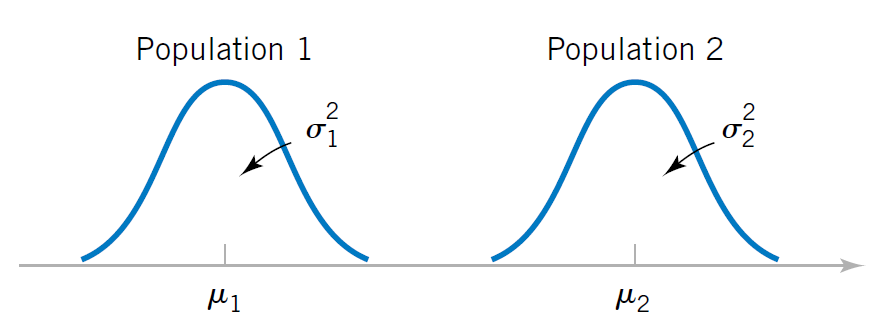
\includegraphics[width=.5\textwidth]{../img/two_population_model}
      \ppagenote{Two models image from D.C. Montgomery "Applied Statistics and Probability for Engineers", Wiley 2003}
    \end{center}
  \end{columns}
\end{frame}

\begin{frame}[t]{Modeling the cutting process}{Comparing Errors}
    \begin{center}
      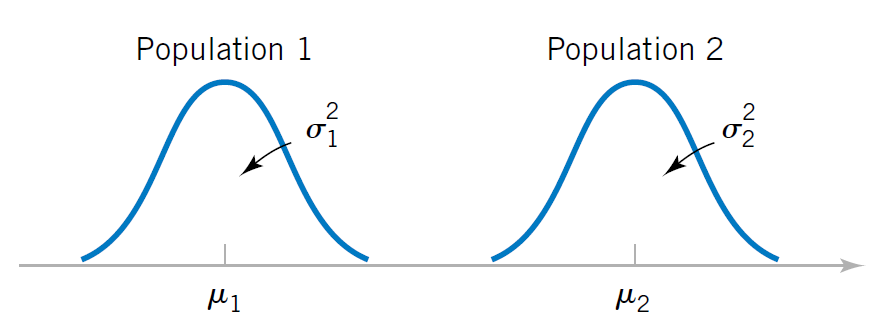
\includegraphics[width=.4\textwidth]{../img/two_population_model}
      \ppagenote{Two models image from D.C. Montgomery "Applied Statistics and Probability for Engineers", Wiley 2003}
    \end{center}

    The sum of two normal variables also follow a normal distribution. So, we can describe the difference between the cutting errors as the random variable $e_{\text{diff}}  = (e_{\text{old}} - e_{\text{new}})$.\bigskip

    Because $e_{\text{diff}}$ also follows a normal distribution, we can use the null hypothesis method to test the difference of the two methods:
    \begin{itemize}
      \item $H_0: e_{\text{diff}} = 0$
      \item $H_1: e_{\text{diff}} \neq 0$
    \end{itemize}
\end{frame}

\subsection{General Statistical Model}
\begin{frame}{A General Model for Comparing two Samples}
  Using the ideas from the previous example, let's describe a general statistical model to use when we want to test if two methods are quantitatively different.\bigskip

  Consider that we measure some observed value ($y$) taken from one of several methods ($i = 1, 2,\ldots$), we understand that the value comes from some distribution with mean $\mu_i$, at it will also have an error ($\epsilon$) away from that mean, which is different for each observation. So we describe the $j$-th observation taken from the $i$-th method as

  \begin{equation*}
    y_{ij} = \mu_i + \epsilon_{ij}\begin{cases}i=1,2\\j=1,\ldots,n_i\end{cases}
  \end{equation*}
\end{frame}

\begin{frame}{Statistical Models}{Two population Model}
  \begin{equation*}
    y_{ij} = \mu_i + \epsilon_{ij}\begin{cases}i=1,2\\j=1,\ldots,n_i\end{cases}
  \end{equation*}\medskip

  Under this model for the observed variable ($y_{ij}$), we assume that the residuals $\epsilon_{ij}$ are independent and follow $\mathcal{N}\left(0,\sigma_i^2\right)$. Under these assumptions, the populations of the two samples look like this:

  \begin{center}
    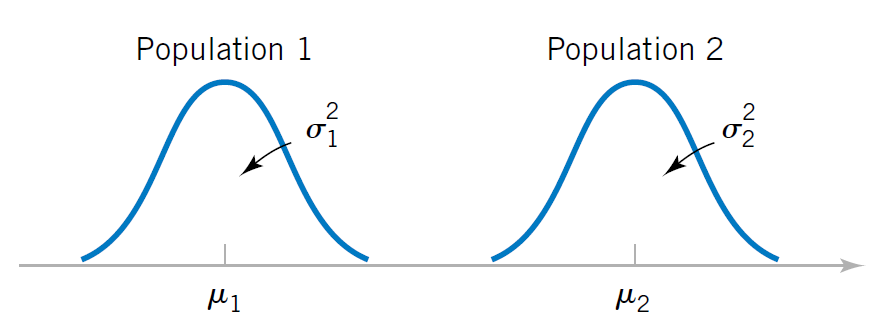
\includegraphics[width=.5\textwidth]{../img/two_population_model}
  \end{center}
\end{frame}

\begin{frame}{Comparison of two means}{Null and Alternate Hypotheses}

What should be the observed variable $y$? The goal of this experiment is to measure if the new method produces steel rods closer to the nominal value. In this case, a possible response variable would be the \structure{absolute error}, e.g., $y = |\ell - \ell_{nominal}|$.\bigskip

Keeping in mind our statistical model, we can build the hypothesis around the \structure{mean} of the absolute error ($\mu_i$). In that case, we can state the null and alternate hypotheses as:
\begin{equation*}
\begin{cases}
H_0: \mu_1 - \mu_2 = 0\\
H_1: \mu_1 - \mu_2 < 0
\end{cases}\ \ \ \mbox{\textbf{or, equivalently, }}\ \ \ \ \ \ \begin{cases}
H_0: \mu_1 = \mu_2\\
H_1: \mu_1 < \mu_2
\end{cases}
\end{equation*}
\medskip
\end{frame}



\begin{frame}{Comparison of two means}{Calculating the statistic}

  Lets assume (for the moment) that the variance of the process is unknown but similar for both systems. Since it is unknown, we have to estimate the variance from the sample data. As assume $\sigma^2_1\approx\sigma^2_2$, we can use the pooled variance estimator:

\begin{equation*}
s_p^2 = \frac{\left(n_1-1\right)s_1^2+\left(n_2-1\right)s_2^2}{n_1+n_2-2}
\end{equation*}
\bigskip

Based on this estimator and the stated assumptions, we calculate the T statistic:
\begin{equation*}
T = \frac{\left(\bar{y_1} - \bar{y_2}\right) - \left(\mu_1 - \mu_2\right)}{s_p\sqrt{\frac{1}{n_1} + \frac{1}{n_2}}}\sim t^{\left(n_1+n_2-2\right)}
\end{equation*}
\end{frame}

\subsection{Calculation of the Statistic}

\begin{frame}
{Back to the Steel Rods Example}
{Calculation of the Rejection threshold}

If we recall our working hypotheses for the steel rod example:

\begin{equation*}
\begin{cases}
H_0: \mu_1 - \mu_2 = 0\\
H_1: \mu_1 - \mu_2 < 0
\end{cases}
\end{equation*}

\noindent we have that, \underline{under $H_0$}:

\begin{equation*}
t_0 = \frac{\left(\bar{y_1} - \bar{y_2}\right) - \cancelto{0}{\left(\mu_1 - \mu_2\right)}}{s_p\sqrt{\frac{1}{n_1} + \frac{1}{n_2}}} = \frac{\left(\bar{y_1} - \bar{y_2}\right)}{s_p\sqrt{\frac{1}{n_1} + \frac{1}{n_2}}}\sim t^{\left(n_1+n_2-2\right)}
\end{equation*}

We'll reject $H_0$ at the $(1-\alpha)$ confidence level if $t_0\leq t^{(n_1+n_2-2)}_{\alpha/2}$
\end{frame}

\begin{frame}
{Back to the Steel Rods Example}
{Statistic Test Parameters}

  Remember that we need to decide \structure{three parameters} that will specify the statistical test:

  \begin{itemize}
    \item {\bf Significance level}: The probability of a {\bf Type I error}. Let's assume that the desired significance level is $\alpha = 0.05$.\bigskip

    \item {\bf Power}: The probability of a {\bf Type II Error}. Let's assume that the desired sensitivity is $1 - \beta = 0.8$.\bigskip

    \item {\bf Meaningful difference}: What is the minimum difference between the two methods that we are interested in detecting? Let's assume $15cm$.
  \end{itemize}\bigskip

The values for these variables depend on the needs of the specific experiment and/or application.

\end{frame}

%%%%%%%%%%%%%%%%%%%%%%%%%%%%%%%%%%%

\begin{frame}[fragile]{Calculating the Statistic}
Computationally, we can perform the t-test for comparing the means of two independent populations by:
\bigskip
{\smaller
\begin{verbatim}
> y <- read.table("steelrods.csv", header = TRUE)
> t.test(y$Length.error ~ y$Process, alternative = "less",
+        mu          = 0, var.equal   = TRUE, conf.level  = 0.95)

data:  y$Length.error by y$Process
t = -14.312, df = 32, p-value = 9.244e-16
alternative hypothesis: true difference in means is less than 0
95 percent confidence interval:
      -Inf -7.156884
sample estimates:
mean in group new mean in group old
         7.782353         15.900000
\end{verbatim}}
\end{frame}

%=====

\begin{frame}[fragile]{Comparison of two means}{Testing the assumptions}


\begin{columns}[T]
  \column{0.7\textwidth}

  The assumptions of the test must be verified. In this particular case:


  {\smaller
\begin{itemize}
  \item \alert{Normality};
  \item Equality of variances;
  \item Independence.
\end{itemize}

{\smaller
\begin{verbatim}
> qqPlot(y$Length.error, groups = y$Process,
        cex = 1.5, pch = 16,  las = 1,
        layout = c(2, 1))
> shapiro.test(y$Length.error[y$Process == "new"])
# W = 0.92269, p-value = 0.164
> shapiro.test(y$Length.error[y$Process == "old"])
# W = 0.94971, p-value = 0.4519
\end{verbatim}}}

{\bf Reminder:} the t-test is quite robust to mild to moderate violations of the normality of the residuals / groups.
\column{.3\textwidth}
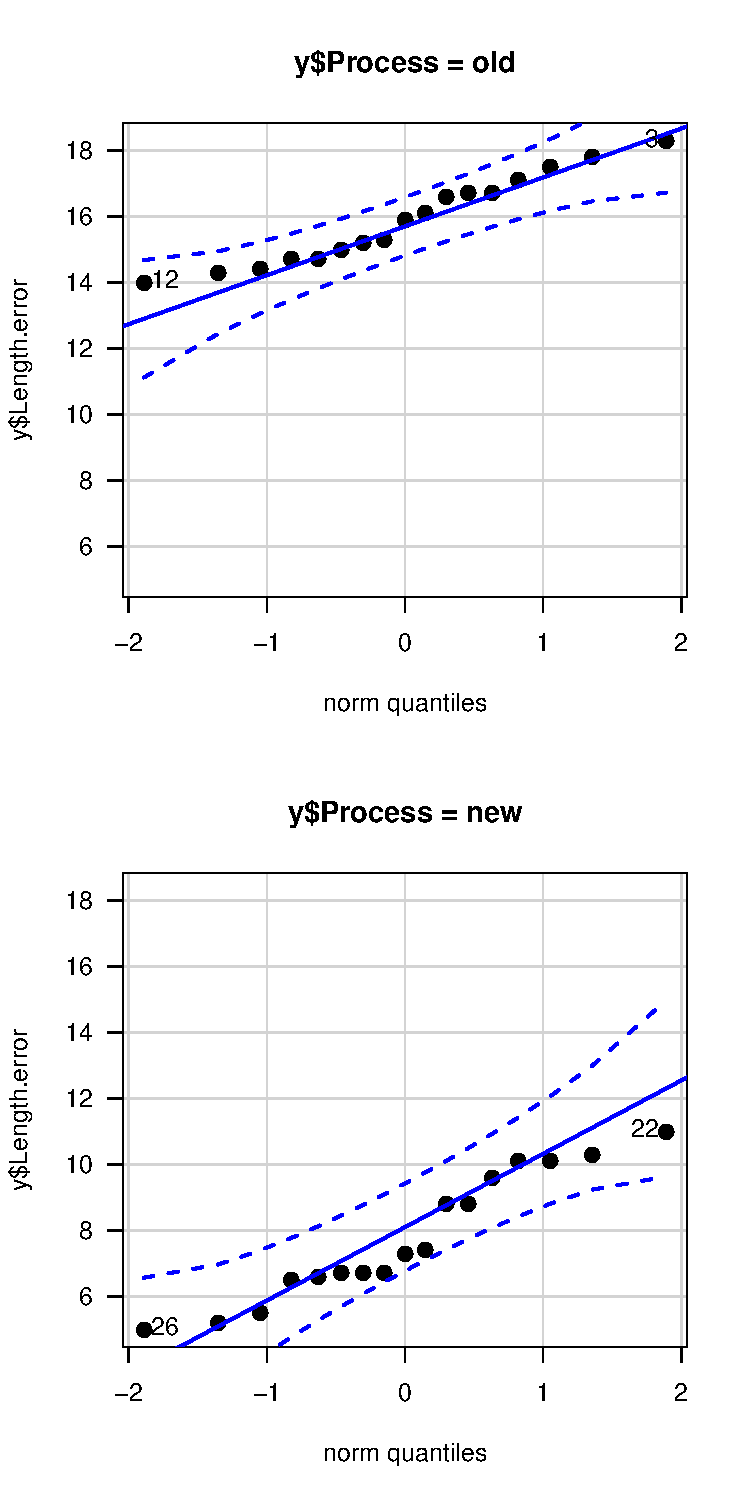
\includegraphics[width=.7\textwidth]{../img/steelrodsqq.pdf}
\end{columns}
\end{frame}

\begin{frame}[fragile]{Comparison of two means}{Testing the assumptions}
The assumptions of the test must be verified. In this particular case:

\begin{columns}[T]
  \column{.7\textwidth}
  {\smaller
    \begin{itemize}
      \item Normality;
      \item \alert{Equality of variances};
      \item Independence;
    \end{itemize}
    {\smaller
\begin{verbatim}
> fligner.test(Length.error ~ Process, data = y)
# Fligner-Killeen:med chi-squared = 1.6837,
# df = 1, p-value = 0.1944

> resid <- tapply(X = y$Length.error,
         INDEX = y$Process,
         FUN   = function(x){x - mean(x)})

> stripchart(x        = resid,
             vertical = TRUE,
             pch      = 16,
             cex      = 1.5,
             las      = 1,
             xlab     = "mean",
             ylab     = "residuals")
\end{verbatim}}}
\column{.3\textwidth}
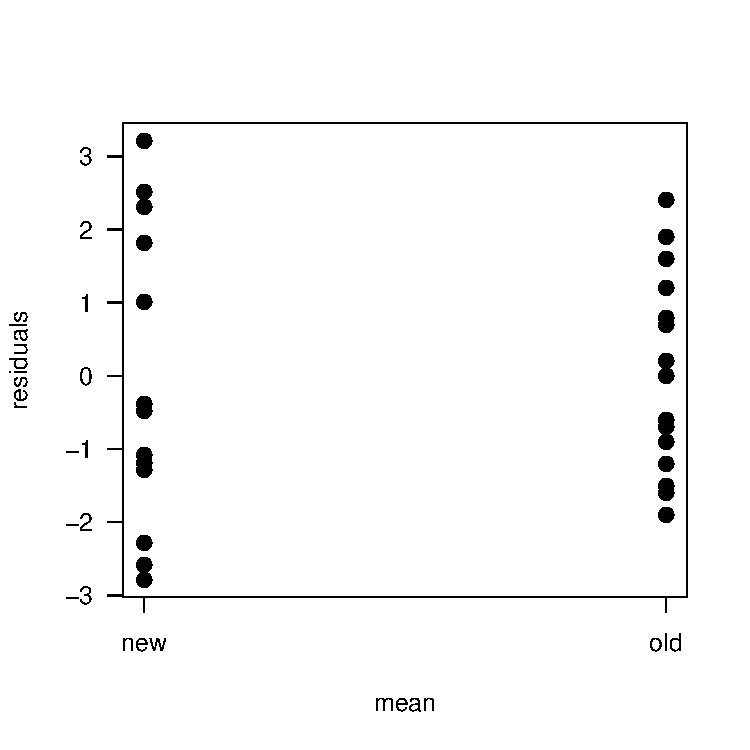
\includegraphics[width=\textwidth]{../img/steelrodsvar.pdf}
\end{columns}
\end{frame}

\begin{frame}
{Comparison of two means}
{Testing the assumptions}
The assumptions of the test must be verified. In this particular case:

{\smaller
\begin{itemize}
  \item Normality;
  \item Equality of variances;
  \item \alert{Independence};
\end{itemize}}
\bigskip

As mentioned in the last class, there is no general test for the independence assumption, and it has to be guaranteed in the design phase.
\bigskip

One can at most test for serial autocorrelation in the residuals using Durbin-Watson's test, but this test is absolutely dependent on the ordering of the observations - very useful to detect ordering-related trends in the residuals, but not much more than that.
\end{frame}

\begin{frame}{Comparison of two means}{Unequal variances}
Suppose now a more general case, in which the variances of the two populations are unknown and cannot be assumed equal.
\bigskip

For this cases, a modification on the t-test called \textit{Welch's t test} is usually employed. The Welch statistic can be calculated as:
\begin{equation*}
  t^*_0 = \frac{\bar{y_1} - \bar{y_2}}{\sqrt{\frac{s_1^2}{n_1} + \frac{s_2^2}{n_2}}}
\end{equation*}
\bigskip

Under the null hypothesis $t^*_0$  is distributed approximately as a $t^{(\nu)}$ distribution, with:
\begin{equation*}
\nu = \frac{\left(\frac{s_1^2}{n_1} + \frac{s_2^2}{n_2}\right)^2}{\frac{\left(s_1^2/n_1\right)^2}{n_1-1} + \frac{\left(s_2^2/n_2\right)^2}{n_2-1}}
\end{equation*}
\end{frame}



\begin{frame}[fragile]{Comparison of two means}{Unequal variances}
To illustrate this technique, let's use the data from the example\footnote[2]{Notice that this would not be necessary, since the data collected in the previous example did not violate the equality of variances assumption.}:
\bigskip

{\smaller{\smaller
\begin{verbatim}
> with(y,
+      t.test(Length.error~Process,
+             alternative = "two.sided",
+             mu = 0,
+             var.equal = FALSE,            %% <- We only change this.
+             conf.level = 0.95))
Welch Two Sample t-test
data:  Length.error by Process
t = -14.312, df = 28.386, p-value = 1.645e-14
alternative hypothesis: true difference in means is not equal to 0
95 percent confidence interval:
-0.09278780 -0.06956515
sample estimates:
mean in group new mean in group old
      0.07782353        0.15900000
\end{verbatim}}}
\end{frame}

%
% \begin{ftst}
% {Comparison of two means}
% {Unequal variances}
% The two-sample Welch t-test for considering unequal variances is usually the first test of choice, since it drops one (often inconvenient) assumption, at a very small cost in terms of power.
% \vone
% Calculating sample sizes for the general case (unequal variances, unequal sample sizes) is not particularly difficult, and can be done for either a \textit{balanced} case (i.e., $n_1 = n_2 = n$) or an optimal, \textit{unbalanced} case (in which $n_1 \neq n_2$).
% \vone
% For the unbalanced case, it is not particularly difficult to prove that the optimal allocation of observation is to keep:
% $$\frac{n_1}{n_2} = \frac{\sigma_1}{\sigma_2}$$.
%
% (if a good estimate of the ratio of variances is available, of course).
% \end{ftst}
%=====

\begin{frame}{Comparison of two means}{Summary}

  To compare an estimator from samples of two populations that (we assume) follow a normal distribution, we set our statistic and the corresponding hypotheses to be the difference of the target variables.\bigskip

  This technique for comparison testing is equally simple and extremely versatile.\bigskip

  Of course, there are cases where this approach does not apply. Next we will see a relatively common case where using the difference of the target variables would lead to a wrong inferential result.
\end{frame}

\section{Paired Testing}
\begin{frame}
  \begin{center}
  {\bf Part II -- Paired Testing}
  \end{center}
\end{frame}

\begin{frame}{Paired Comparison of Two Samples}{Outline}

  In the last part, we studied how to apply the statistical inference method using hypothesis testing to the situation where we want to compare two samples.\bigskip

  In this part, we will study a common special situation, where there is a strong dependency between observations in the samples.\bigskip

  The change in the calculation is very minor, but the results can be very different!
\end{frame}

\subsection{Motivation}
\begin{frame}{Examples of Paired Design}{Paired Design happens when the observations in both samples have strong dependencies.}

  \begin{block}{Example 1: Football shoes}
    Out of two brand of football shoes, you want to measure which one wears out faster.
    \begin{itemize}
      \item You make a team play two games, one with shoe A, one with shoe B. You measure the amount of wear for each player's shoes.
      \item You know that the Foward's shoes will wear much more than the Goalkeeper's shoes.
    \end{itemize}
  \end{block}
  \begin{block}{Example 2: Fuel Efficiency}
    You want to measure if a new kind of fuel is more efficient than an old one.
    \begin{itemize}
      \item You choose 10 cars, fill then with each type of fuel, make then run until they are out of fuel, and measure the distance.
      \item You know that different car types consume fuel at very different rates.
    \end{itemize}
  \end{block}
\end{frame}

\begin{frame}{Computer Science Example}{Comparison of Two Optimization Methods}

A researcher develops a new optimization algorithm (A), and wants to compare its
convergence speed against a method that represents the state-of-art (B).\bigskip

The researcher believes that the proposed algorithm has a theoretical advantage on a {\bf specific family of optimization problems}, so she selects a set of benchmark problems from that family.\bigskip

Both methods are executed on the benchmark set, and the time-to-convergence is measured for each problem. The measurements are made under homogeneous conditions (same computer, same operating conditions, etc).
\end{frame}

\begin{frame}{Computer Science Example}{Consideration for Experiment Design}

In this example, we are taking several problem instances, and running each
of the two algorithms in all instances. Because of the expected variation in
running time, we might want to run one "algorithm-instance" multiple times.\bigskip

This problem has some important questions worth considering:
\bigskip

\begin{itemize}
  \item What is the \structure{estimator} that should be measured in this experiment?
  \item What is one \structure{independent observation} for this experiment?
  \item What is the relevant sample size for the experiment?
\end{itemize}
\bigskip

\begin{block}{}
  Think about the difference between considering \structure{individual runs} as observations and \structure{individual problems} as observations.
\end{block}
\end{frame}


\subsection{Definitions}
\begin{frame}{Paired Experimental Design}{Why is Pairing Necessary?}

  When we consider observations with strong dependencies (players, cars types, benchmark problems), the difference between the observations is a strong source of variation (noise) that is not related to the objective of the experiment.\bigskip

  This variation can, and must, be controlled in the experiment design.\bigskip

  An elegant solution to eliminate the influence of this nuisance parameter is the \textit{pairing} of the measurements by problem:\bigskip

  \begin{itemize}
  \item Observations are considered in pairs (A, B) for each benchmark problem;
  \item Hypothesis testing is done on the sample of ""\textit{differences for a benchmark}";
  \end{itemize}
\end{frame}

\begin{frame}{Paired Experimental Design}{Statistical Model}
Let $y_{Aj}$ and $y_{Bj}$ be the paired observations of the average time for methods A and B, for a problem instance $j$. The \textit{paired difference} of an observation is simply $d_j = y_{Aj} - y_{Bj}$.
\bigskip

If we model our observations as an additive process:
\begin{equation*}
y_{ij} = \underbrace{\mu + \tau_i}_{\mu_i} + \beta_j + \varepsilon_{ij}
\end{equation*}
\noindent where $\mu$ is the grand mean, $\tau_i$ is the effect of the $i$-th method on the mean (A or B), $\beta_j$ is the effect of the $j$-th problem, and $\varepsilon_{ij}$ is the model residual, then:
\begin{equation*}
\begin{split}
d_j &= y_{Aj} - y_{Bj}\\
&= \mu + \tau_A + \beta_j + \varepsilon_{Aj} - (\mu + \tau_B + \beta_j + \varepsilon_{Bj})\\
&= \cancel{\left(\mu +\beta_j - \mu - \beta_j\right)} + \tau_A-\tau_B + \varepsilon_{Aj}-\varepsilon_{Bj}\\
&=\mu_{D} + \varepsilon_j\\
\end{split}
\end{equation*}

\end{frame}

\begin{frame}{Paired Experimental Design}{Hypotheses}
The hypotheses of interest can now be defined in terms of $\mu_D$, e.g.:
\begin{equation*}\begin{cases}
H_0: \mu_D = 0\\
H_1: \mu_D \neq 0
\end{cases}\end{equation*}

And now, we are back to our traditional "single sample hypothesis test". The population of interest is the difference in convergence time for the family of problems under investigation. The test statistic is given by:
\begin{equation*}
  T_0 = \frac{\bar{D}}{S_D/\sqrt{N}}\sim t^{(N-1)}
\end{equation*}
\bigskip

Where $\bar{D}$ is the average of the paired differences, and $N$ is the number of benchmark problems in the experiment.
\end{frame}


\begin{frame}{Paired Experimental Design}{Other Considerations}
Some other important questions worth considering:
\medskip

\begin{itemize}
\item In this example the minimally interesting effect size $\delta^*$ must be expressed in terms of \textit{average time gains across problems} (not within individual instances).
\item The most important sample size to consider in this situation refers to the \textit{number of problem instances}, and not necessarily to the number of within-problems repeated measures;
\item The number of repetitions within each problem will have an impact on the uncertainty associated to each observation (that is, to each value of mean time to convergence for each algorithm on each problem), which will propagate down to the residual variance.
\end{itemize}
\end{frame}



\begin{frame}{Paired Experimental Design}{Summary}

\begin{itemize}
  \item The Paired Design removes the effects of \structure{controllable} nuisance factors from the analysis. (Problem type, personal characteristics, etc)\bigskip

  \item It is strongly indicated in cases with {\bf strong correlations between samples}\\
  (e.g., heterogeneous experimental conditions).
\end{itemize}
\end{frame}

\subsection{Benchmark testing Example}

\begin{frame}{Paired Comparison Example}
Going back to our example, assume the following facts about the desired comparison:\bigskip

\begin{itemize}
\item The benchmark set is composed of seven problem instances ($N=7$);
\item The researcher is interested in finding differences in mean time to convergence greater than ten seconds ($\delta^*=10$) with a power of at least $(1-\beta)=0.8$, using a significance level $\alpha=0.05$;
\item The researcher performs $n=30$ repeated runs\footnote[1]{\tiny Not that this number is necessarily good, but it is generally an easy alternative if you don't want to keep justifying your choices to less statistically-savvy reviewers.} of each algorithm in each problem, from random initial conditions.
\end{itemize}
\end{frame}


\begin{frame}[fragile]{Executing the Paired Analysis}
  {Step 1: load and precondition the data}

\begin{columns}
  \column{0.7\textwidth}
{\smaller{\smaller
\begin{verbatim}
> # Read data from CSV file
> data <- read.table("benchmark.csv", header=T)

# Change the type of the "Problem" variable
#                 from "number" to "Factor"
> data$Problem <- as.factor(data$Problem)

# Summarize within-problem observations by mean
> aggdata <- aggregate(Time ~ Problem:Algorithm,
+                      data = data, FUN  = mean)
> summary(aggdata)
 Problem Algorithm      Time
 1:2     A:7       Min.   : 37.63
 2:2     B:7       1st Qu.:109.45
 3:2               Median :178.73
 4:2               Mean   :175.48
 5:2               3rd Qu.:245.25
 6:2               Max.   :296.79
 7:2
\end{verbatim}}}
\column{0.3\textwidth}
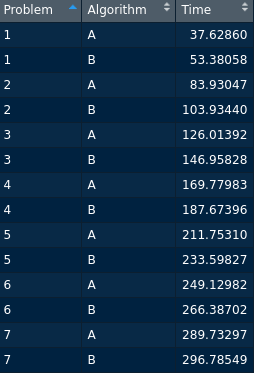
\includegraphics[width=1\textwidth]{../img/steelrods_summarytable}
\end{columns}
\end{frame}

\begin{frame}{Executing the Paired Analysis}{Influence of the problem type in the results}
      Note that the difference between problems is bigger than the difference between methods.
  \begin{center}

  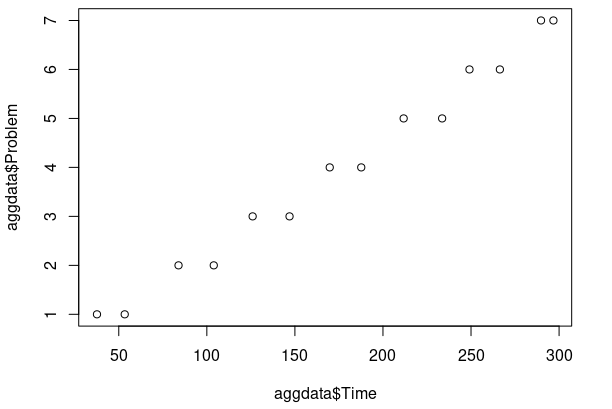
\includegraphics[width=.6\textwidth]{../img/steelrods_timediff}
  \end{center}
\end{frame}

\begin{frame}[fragile]{Executing the Paired Analysis}{Step 2: analysis}
  {\smaller
\begin{verbatim}
> # Perform paired t-test
> t.test(Time ~ Algorithm, data = aggdata,
+        paired = TRUE)           #  <-- To do a paired test, just change here.

Paired t-test
data:  Time by Algorithm
t = -9.1585, df = 6, p-value = 9.54e-05
alternative hypothesis: true difference in means is not equal to 0
95 percent confidence interval:
 -21.85862 -12.64118
sample estimates:
mean of the differences
               -17.2499
\end{verbatim}}
\end{frame}



%=====

\begin{frame}[fragile]
{Executing the Paired Analysis}
{Step 2: Alternate calculation}

{\smaller
\begin{verbatim}
# Create an array with the difference per problem, and perform one-sample test.
> difTimes <- aggdata$Time[1:7] - aggdata$Time[8:14])
> t.test(difTimes)

One Sample t-test
data:  difTimes
t = -9.1585, df = 6, p-value = 9.54e-05
alternative hypothesis: true mean is not equal to 0
95 percent confidence interval:
 -21.85862 -12.64118             # Same result!
sample estimates:
mean of x
 -17.2499
\end{verbatim}}
\bigskip

{\bf Check your understanding:} Why is the paired test on two samples equivalent to the one sample test on the difference vector of the samples?
\end{frame}

\begin{frame}[fragile]{Paired Analysis}{Step 3: Testing the assumptions}
  As usual, you should test the normality and variance of your data, and guarantee the independence of the observations. Let's check the normality test.
  \begin{columns}
    \column{0.6\textwidth}
{\smaller{\smaller
\begin{verbatim}
> shapiro.test(difTimes)
Shapiro-Wilk normality test
data:  difTimes
W = 0.8387, p-value = 0.09655

# Redo test without outlier
> indx <- which(difTimes == max(difTimes))
> t.test(difTimes[-indx])$p.value
[1] 6.179743e-06
> t.test(difTimes[-indx])$conf.int
[1] -21.41856 -16.48037
\end{verbatim}}}
\column{0.35\textwidth}
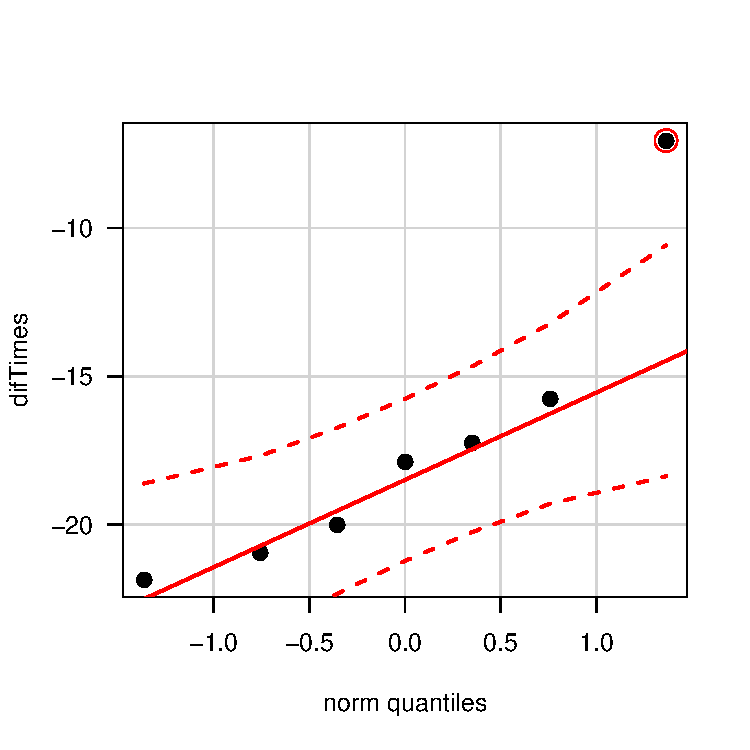
\includegraphics[width=.8\textwidth]{../img/soltimesqq.pdf}
\end{columns}
The normality test showed one big outlier. It does not invalidate the test, but
it should be examined. You might learn something important!
\end{frame}



%=====

\begin{frame}[fragile]{Why is Pairing Important?}{What happens if we ignore the dependency between observations?}
{\smaller
\begin{verbatim}
> t.test(Time ~ Algorithm, data = aggdata)

Welch Two Sample t-test
data:  Time by Algorithm
t = -0.3609, df = 11.993, p-value = 0.7245
alternative hypothesis: true difference in means is not equal to 0
95 percent confidence interval:
 -121.40320   86.90341
sample estimates:
mean in group A mean in group B
       166.8527        184.1026
\end{verbatim}}

If we don't take into account the large variation among problems, {\bf it will hide
variation between the two methods.}

% In a similar way, if we fail to recognize the similarity between observations, it is possible to artificially inflate $\alpha$ by \alert{pseudo-replication}.
\end{frame}

\begin{frame}{Why is Pairing Important?}{A visual Comparison}
  \begin{columns}
    \column{0.5\textwidth}
    \begin{center}
      Paired Samples
    \end{center}
    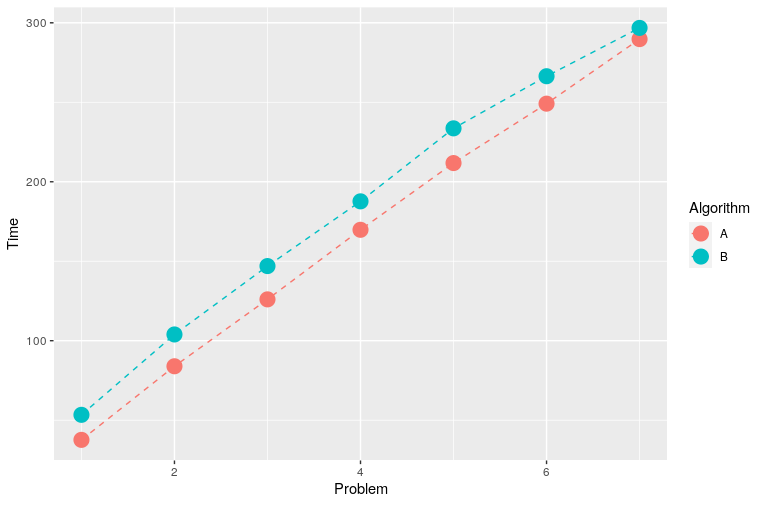
\includegraphics[width=\textwidth]{../img/2samples_paired}
    \column{0.5\textwidth}
      \begin{center}
        Unpaired Samples
      \end{center}
    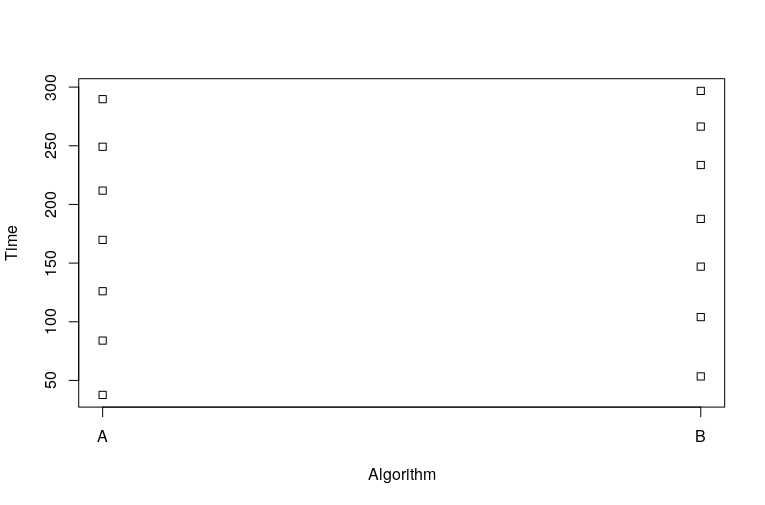
\includegraphics[width=\textwidth]{../img/2samples_unpaired}
  \end{columns}
\end{frame}

%=====
%
% \begin{ftstf}
% {Comparison of two means}
% {Paired design}
% Paired designs can require smaller sample sizes for equivalent power in cases where the between-units (in our example, the between-problems) variation is relatively high;
% \vhalf
% More specifically, if the within-level variation is given by $\sigma_\epsilon$ and the between-units variation is $\sigma_u$, we have that, for large enough $N$\\(e.g., $N\geq 10$),
% \beqs
% \frac{N_{\mbox{\tiny unpaired}}}{N_{\mbox{\tiny paired}}}\approx\sqrt{2\left[\left(\frac{\sigma_u}{\sigma_\epsilon}\right)^2+1\right]}
% \eqs
% \vhalf
% Failure to consider inter-unit variability can result in the masking of relevant effects by the nuisance factor.
% \vhalf
% Similarly, failure in recognizing the dependence structure of within-unit measurements yields tests with artificially inflated degrees of freedom, which results in the inflation of the effective value of $\alpha$.
% \end{ftstf}

%% My slide: A few more examples of paired testing.

\section{Conclusion}
\begin{frame}
  \begin{center}
    {\bf Conclusion}
  \end{center}
\end{frame}

\begin{frame}{Summary}
  \begin{itemize}
    \item In the Last class, we described the Null Hypothesis testing method to perform {\bf Statistical Inference} on a population parameter from a single sample;
    \bigskip

    \item In this cless, we generalize this procedure to a common situation, where we want to compare two samples regarding a population parameter;
    \bigskip

    \item The {\bf Two Sample Hypothesis Testing} uses inference on a statistic based on the \structure{difference between sample estimators}.\bigskip

    \item When there is a high correlation between the observations of each sample, it is important to perform the \structure{pairing} of the observations.
  \end{itemize}
\end{frame}

\subsection{Report 02}

\begin{frame}{Report 2}{Design, Execute and Analize a Scientific Experiment}
  In this report, you must choose a simple experiment to design, perform and analyze the results. Like in Report 1, your report must have:
  \begin{itemize}
    \item {\bf Introduction}: Description of Scientific Question;
    \item {\bf Experiment Design}: Plan of data collection \structure{and analysis}
    \item {\bf Data Collection:} Report on the data and results;
    \item {\bf Analysis:} \structure{Conclusion based on hypotheses and statistic};
  \end{itemize}

  \begin{alertblock}{Important Notes}
    \begin{itemize}
      \item Use techniques of \structure{Statistical Inference} to analyze the results;
      \item In the Experiment Design section, describe the hypotheses used, and the variable of interest;
      \item In the Analysis section, do not forget to test the inferential assumptions (normality, variance, etc);
      \item Remember to follow practices of reproducible science!
    \end{itemize}
  \end{alertblock}
\end{frame}

\begin{frame}{A note about data re-use}
  Because this report is very similar to Report 01, a natural question is "Can I use the same data as in the first report, and just change the analysis?".\bigskip

  \alert{The short answer is {\bf NO}}.\bigskip

  The idea of experimental design is that the setup of the experiment, including the choice of variable, statistic, hypotheses, etc, should guide the data collection, not the other way around. \structure{Choosing the analysis {\bf after} data collection is an easy way to bias the results}.

  \begin{exampleblock}{How you can use your initial data:}
    You can, however, use your previous experiment data to guide the design of the new experiment. For example, you can use it to estimate variance, reasonable values for the hypotheses, etc.
  \end{exampleblock}
\end{frame}

\subsection{Related Reading}
% \begin{frame}{Related Reading}
% \end{frame}

%%%%%%%%%%%%%%%%%%%%%%%%%%%%%%%%%%%%%%%%%%%%%%%%%%%%%%%%%%%

\subsection{Pre-lecture Comments}

\begin{frame}{Comments on Report 01}
  \begin{itemize}
    \item I gave a quick look at the reports, but the full grading will take a bit of time, so please be patient;
    \item In general, everyone did great reports, I am very happy with the results;
    \item However, there were some common mistakes:
    \begin{itemize}
      \item Many people did not include code for reproducibility; or the data used in the analysis; \alert{Non-reproducible reports will receive a lower grade}.
      \item A few students did not submit reports in PDF; \alert{The main file of the report MUST be a PDF}
      \item One student asked to use secret experimental data in the report; \alert{It is acceptable, but I recommend against it in the future};
    \end{itemize}
  \end{itemize}
\end{frame}


%%%%%%%%%%%%%%%%%%%%%%%%%%%%%%%%%%%%%%%%%%%%%%%%%%%%
\section{Backmatter}
\begin{frame}{About these Slides}
  These slides were made by Claus Aranha, 2022. You are welcome to copy, re-use and modify this material.
  \bigskip

  These slides are a modification of "Design and Analysis of Experiments (2018)" by Felipe Campelo, used with permission.
  \bigskip

  Individual images in some slides might have been made by other
  authors. Please see the following references for those cases.
\end{frame}

\begin{frame}[allowframebreaks]{Image Credits}
  \printnotes
\end{frame}

\end{CJK}
\end{document}
